\section{Usability Tests}
\subsection{MapReduce with Distributed Hash Tables}
To test both performance and usage of the distributed hash tables a MapReduce framework was implemented. MapReduce was chosen because it was convenient to have an distributed data type as underlying structure as well as the goal of the framework to easily work with parallelism is similar to the goal of the implemented library. What program that was implemented is not the focus, other types of programs could have been used for testing.

\subsection{Functionality Provided}
\subsubsection{Automatic Sorting \& Process Distribution}
One of the important steps in the MapReduce is to sort keys in each step and distribute data between different working nodes. Each step in the implemented MapReduce that holds data contains of one distributed hash tables, in each level the working nodes send it's output to the next. Sorting and distribution will happen automatically because of how the distributed hash table inserts values.\\ 

The distributed hash table inserts incoming data by placing all values with the same key at same place. The fact that different keys all ready are distributed among many workers in the hash table result in good distributed between nodes by default as long as there is more than a few different keys. \\

Distributed arrays could be used for this MapReduce implementation with similar result but because of that the interface in MapReduce always use key-value pairs hash tables works out of the box.

\subsection{Functionality Not Provided}
\subsubsection{Multiple Values per Key}
Instead of having only one value mapped to each key each key in a MapReduce stage needs to store multiple values and be able to dynamically append values. This was not a supported features when starting the evaluation. At the bottom level each hash-entry was changed to be a link-list instead of only consist of one value, no old functionality was changed but methods to extend and extract many values from one specific hash entry was added.

\subsubsection{Advanced Constructs In Workers}
Much of the work done in the MapReduce steps are done at the bottom level (in the workers). For example when users provided a map and a reduce functions and all the message sending between each steps all have to be done from the bottom level. It was clear that at this stage the functionality needed could not be created outside and inserted into the distributed hash table class, mostly because bottom level are abstracted away from the outside. The distributed hash table was extended with one mapper and one reducer method to each handle one step in the MapReduce implementation. Preferable one would want an interface where these function could be inserted instead of implemented directly into the library.

\pagebreak

\subsection{MapReduce Programs}
With a correctly implemented MapReduce framework creating new programs should be easy. The user provides one map and one reduce function and prepare the input. This MapRecude implementation provide some functionality to help the user with the setup such as an Encore graph representation and hashing functions for different data types. Some example program has been implemented to showcase what and how one could use the Encore MapReduce implementation with the distributed hash tables.

\begin{figure}[h]
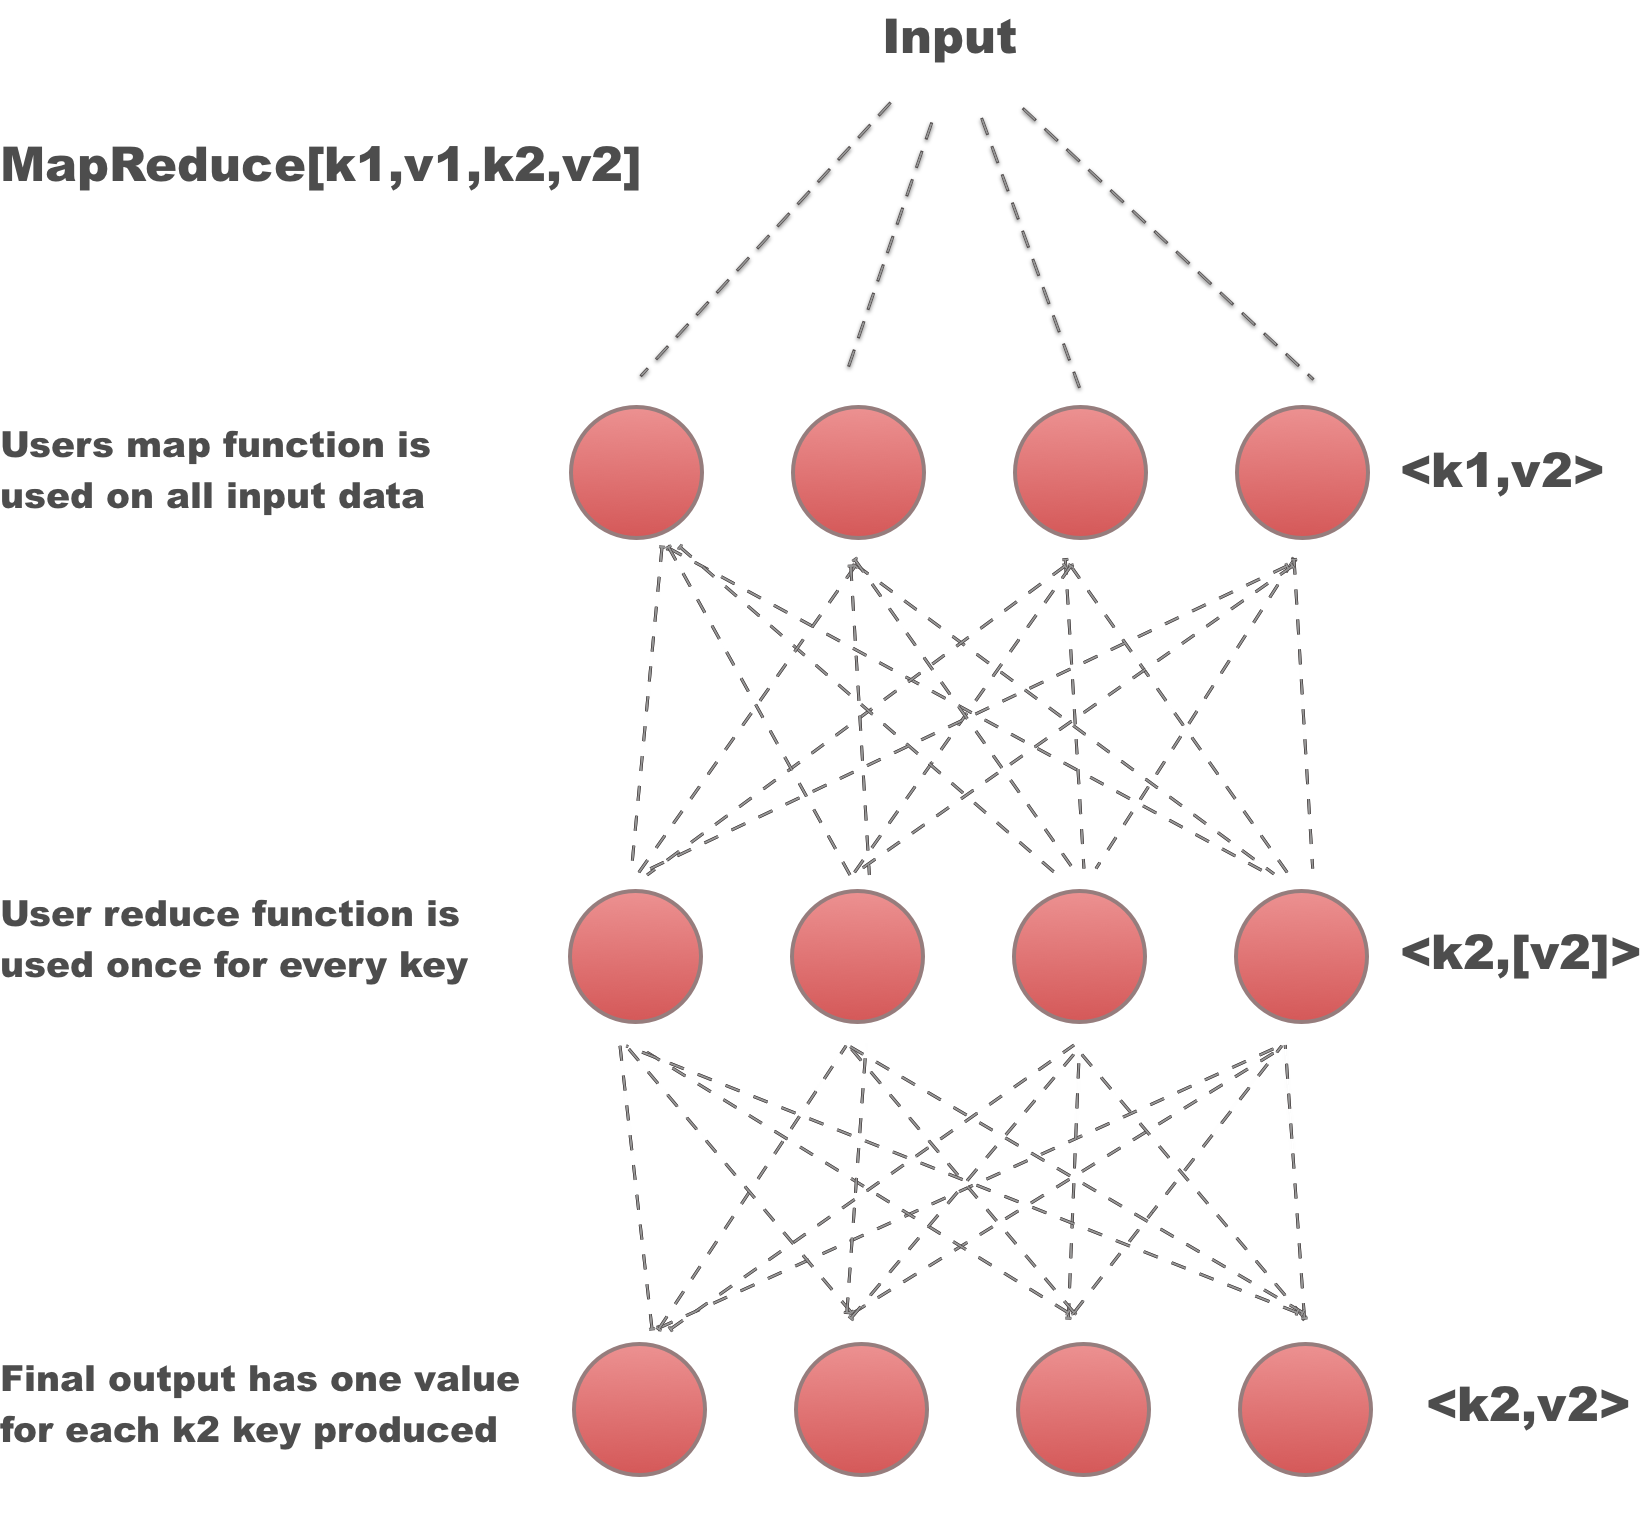
\includegraphics[width=12cm]{images/MapReduceFigure}
\\Figure(4): A simplified view of the MapReduce process, each layer consist of a distributed hash table. The figure only shows one run, some algorithms need many iterations to complete the task, if that is the case the types k2 and v2 match the types k1,v1.
\end{figure}
\pagebreak

\subsubsection{Word Count}
\begin{lstlisting}
fun map(key:int,value:String) : [(String,int)]
    var words = value.to_lower().split(" ")
    var result = new[(String,int)](|words|)
    repeat i <- |words| do
        result(i) = (words(i),1)
    end
    result
end
\end{lstlisting}
\begin{lstlisting}
fun reduce(key:String,values:[int]) : (String,int)
    var sum = 0
    for value <- values do
        sum += value
    end
    (key,sum)
end
\end{lstlisting}

First the map and reduce function is created, then the programmer inserts the input-data to a distributed hash object as well as create a new MapReduce object with the correct type definition. The four different types used in the MapReduce object k1,v1,k2,v2 can be extracted from the map and the reduce functions as seen bellow.

\begin{lstlisting}
map(k1,v2) -> [(k2,v2)]
reduce(k2,[v2]) -> (k2,v2)
\end{lstlisting}

To run a MapReduce job the programmer calls the run method on the MapReduce object with the distributed hash table input, the map and the reduce function as parameters. stringID is a hashing function for the k2 type and is needed in the initialization for the MapReduce object. 

Returned from the run method is a distributed hash table with the result stored in k2-v2 format. In the Word Count program result is different words mapped to how many times that word appears in the input text. 

\begin{lstlisting}
var mapReduce = new MapReduce[int,String,String,int](stringID)
var graph = mapReduce.run(consume graph, map, reduce)
\end{lstlisting}

The result could be continue to worked with as the function returns a distributed hash table object. Single values could be extracted from the hash table with the get(key) method, if all values are wanted the user could loop trough the distributed hash table with keys generated from the .keys() method. 
\pagebreak

\subsubsection{Shortest-path with Parallel Breadth-first Search}
\begin{lstlisting}
fun map(key:int,value:Node) : [(int, Node)]
    if value.color == 1 then
        value.color = 0
        var adjList = value.adjList
        var result = new[(int,Node)](|adjList|+1)
        repeat i <- |adjList| do
            var id = adjList(i).id
            var dist = new Node(-1) -- Distance Node
            dist.distance = value.distance + 1
            dist.color = 1
            result(i) = (id,dist)
        end
        result(|adjList|) = (key,value)
        result
    else
        [(key,value)]
    end
end
\end{lstlisting}
\begin{lstlisting}
fun reduce(key:int, values:[Node]) : (int, Node)
    var dmin = 100
    var node = new Node(-1)
    var color = 2
    for d <- values do
        if d.id >= 0 then
            node = d
        else
            if d.distance < dmin then
                dmin = d.distance
            end
        end
        if d.color < color then color = d.color end
    end
    if node.distance > dmin then node.distance = dmin end
    node.color = color
    (key,node)
end
\end{lstlisting}
\pagebreak

\section{Performance Tests}
When testing the implementation of Bigvars focus has been on the distributed hash tables. The structure different between the hash tables and the distributed arrays is not enough to make important difference. If one shows good result the principle with distributed data types is credited and both are promising. Currently do the distributed hash tables have more implemented functionality. The implemented MapReduce program (See previously section) is implemented with distributed hash tables but could have been written with an distributed arrays as well. \\ 

\subsection{Flame Graphs}
Flame Graph is a tool to measure program performance. It approximates for how long specific functions holds the CPU during the program execution. The tool achieve this by by tracing the stack and taking samples. Flame Graphs is great for the programmer to get an overview of where in the program time is spent and also see the stack structure. Flame Graphs is an open source tool and was created by Brendan Gregg \cite{flamegraph}.\\

In the Flame-Graph diagram each box on the y-axis represents one the stack-frame and the width of the boxes percentage of the program execution that stack frame was there, the boxes is sorted alphabetically\cite{flamegraph}.
\subsubsection{Can performance be optimized? - What to look for}

\begin{itemize}
\item \blindtext How expensive is to rehash? Worth to invest in more memory?
\item \blindtext How is creating many empty futures affecting performance? 
\item \blindtext How much time is spend sending messages? is it worth optimizing?
\end{itemize}

\subsection{Overview Performance Test}
This test use the implemented MapReduce Framework with an parallel breadth first search algorithm \cite{mapreduce}, it finds how many hopes every node is from the starting node in an undirected none weight graph (see section 7.1.4 for code). \\ 

\begin{figure}[h]
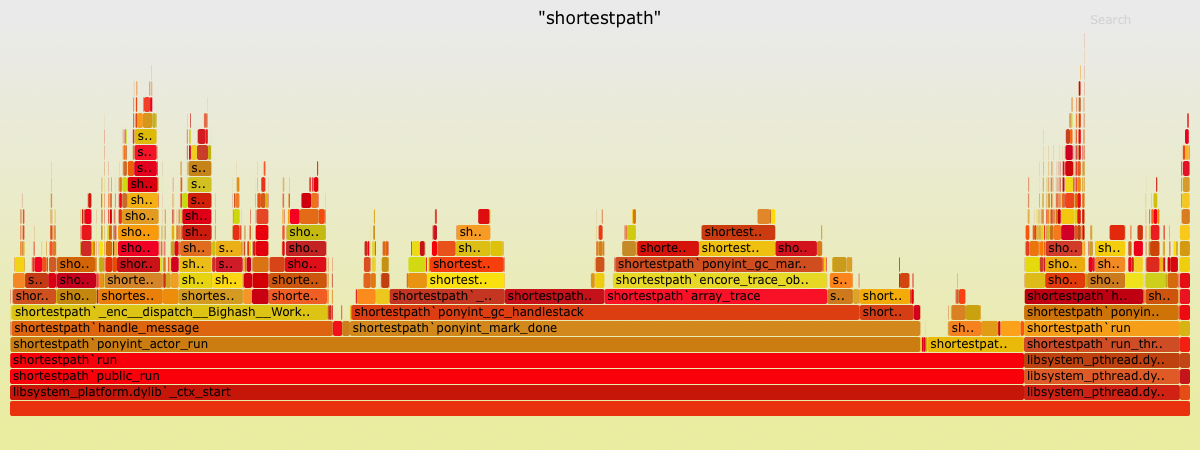
\includegraphics[width=12cm]{images/FlameBig}
\end{figure}

\subsubsection{Result}
Most flame-graphs generated when using the shortest-path algorithm was very similiar even with different number of nodes. The one above graph is running shortest-path on a graph with 50 000 nodes. The evaluating shows as expected that the user map and reduce function take up little of the actually running time of the program, 5,44\% and 5,45\%. Note that this will vary much depending on how heavily the user functions is but no matter what the other steps in MapReduce will take take up time.

\subsubsection{Code Changes}
After inspection different flame-graphs and the running times with different parameters some changed was made in hope of optimize the performance of the distributed hash tables. Optimizing the hash tables will speed up MapReduce programs because it is the underlying data structure used.

\subsubsection{Extracting Values}
Methods that inserts and extract values from the distributed hash tables takes notable time, after examine those closer a better way of extracting values from the link-list was found, this increased the speed of the algorithm slightly.

\subsubsection{Optimizing Message Sending}
For every key-value pair the user map function returns a message is sent to the next stage in the MapReduce program. When using the distributed hash table one would sometimes, like in this case want to batch many pairs together and send them in one message instead of many separate massage, methods for this functionality was added and tested used in the MapReduce map step. All messages now contain an array with many pairs instead of a single pair. \\

This resulted in a lot less massage sending but the trade off is that all pairs instead needs to be sorted before. In the current implementation a link-list is created for each worker, the length of the result from each map function is unknown therefor arrays can be tricky to work with. For every pair a key is hashed (hashing was also needed before this optimization) and the values are inserted in the correct linked list. Lastly all the values are extracted from the link-list and inserted to an array to later be sent to a worker. For each batch of pairs only one massage is sent to each worker, The result are not as great as hoped. \\ insert diagrams here

\subsection{Parallel Performance Test}
\subsubsection{result}

\section{Shortcomings}
\subsubsection{Distribution}
Encore is scalable to machines with hundreds or maybe thousands of cores \cite{encore}, unfortunately most personal computer 2017 only have 4 or 8 cores. Because of the fact that the current implementation of distributed hash tables only can be distributed on one single machine operation that are able to run in parallel is not that many. To achieve full performance benefit from distributed data types one would want as many working nodes as possible, to achieve this distribution between machine is probably a good idea. 

\subsubsection{Time limit}
This distributed data type Library was Implemented during time period of 10 weeks and is a part of this bachelor thesis. Everything is not perfect and compered to other similar implementation not a lot of time have been spent on optimizing performance.

\subsubsection{Functionality of Distributed Arrays}
Because of the decision to focus on the distributed hash tables instead of distributed arrays, some designed functionally was not implemented for the distributed arrays. like reference creation, automated redistribution and programmer defined parameters.
\pagebreak